\documentclass[11pt,a4paper]{article}

\usepackage[margin=2.5cm]{geometry}
\usepackage[T1]{fontenc}
\usepackage{graphicx}
\usepackage{booktabs}
\usepackage{longtable}
\usepackage{tabularx}
\usepackage{array}
\usepackage{xcolor}
\usepackage{float}
\usepackage{enumitem}
\usepackage{pgfgantt}
\usepackage{fancyhdr}
\usepackage[hidelinks]{hyperref}

\graphicspath{{../diagrams/}}
\setlist{itemsep=2pt,topsep=4pt}
\setlength{\parskip}{4pt}
\setlength{\parindent}{0pt}
\renewcommand{\arraystretch}{1.15}
\pagestyle{fancy}
\fancyhf{}
\fancyhead[L]{\small CampusShare -- Capstone Project Proposal}
\fancyhead[R]{\small Individual Project}
\fancyfoot[C]{\thepage}

% ---------- Editable placeholders ----------
\newcommand{\studentname}{Swapnil Nag Swachha}
\newcommand{\studentid}{IT24001}
\newcommand{\university}{Mawlana Bhashani Science and Technology University}
\newcommand{\department}{Department of Information and Communication Technology}
\newcommand{\instructor}{Dr. Ziaur Rahman}
\newcommand{\submissiondate}{27 October 2026}

\begin{document}

% ---------- Title page ----------
\begin{titlepage}
\centering
\vspace*{1.5cm}
{\large \university\par}
\vspace{4pt}
{\large \department\par}
\vspace{2cm}
{\Huge\bfseries CampusShare\par}
\vspace{8pt}
{\Large A Campus Resource Borrowing and Sharing Platform\par}
\vspace{1.2cm}
{\large Individual Capstone Project Proposal\par}
\vspace{2.5cm}
\begin{tabular}{ll}
\textbf{Student Name:} & \studentname\\[4pt]
\textbf{Student ID:} & \studentid\\[4pt]
\textbf{Supervisor:} & \instructor\\[4pt]
\textbf{Submission Date:} & \submissiondate\\
\end{tabular}
\vfill
{\small Status: project proposal, system design and an initial UI prototype. The full application is planned for future development.\par}
\end{titlepage}

\tableofcontents
\newpage

% ---------- 2 Abstract ----------
\section*{Abstract}
\addcontentsline{toc}{section}{Abstract}
University students often need items for a short time, such as a scientific calculator for an exam, a lab coat for a practical session, or a textbook for one chapter. Buying these items for brief use is costly, while many other students own the same items and use them rarely. This proposal presents CampusShare, a simple web application that lets students list items they are willing to lend, browse and search available items, send borrowing requests, and track request and borrowing status. An administrator manages users, item categories, and reported items. The system is planned as a layered Java Spring Boot application with Spring MVC, Spring Data JPA, MySQL, and Thymeleaf views. The project follows the Incremental Model and is scheduled over six weeks for one student. This document contains the requirements, design diagrams, database design, schedule, testing strategy, and an initial UI prototype. The full backend has not yet been implemented.

% ---------- 3 Introduction ----------
\section{Introduction and Background}
Students on a campus share many small needs: textbooks, calculators, stationery, lab accessories, and sports equipment. Many of these items are used only during certain weeks of a semester. Informal sharing through messaging groups or notice boards exists, but requests are easily lost, availability is unclear, and nobody can see who has borrowed what.

CampusShare proposes a small, dedicated platform for this purpose. It is not intended to be a commercial marketplace. Its aim is to give students one organised place to offer items, find items, and manage borrowing in a clear and traceable way.

% ---------- 4 Problem Statement ----------
\section{Problem Statement}
Sharing items between students is currently informal and unstructured. As a result:
\begin{itemize}
  \item students cannot easily find out which items are available on campus;
  \item borrowing requests are made through scattered messages and are easy to miss;
  \item owners cannot easily track who has their item and when it should be returned;
  \item there is no simple way to report a problem with a listing or to record feedback after borrowing.
\end{itemize}
A simple web-based system with clear request statuses is needed to organise this process.

% ---------- 5 Aim and Objectives ----------
\section{Aim and Objectives}
\textbf{Aim:} To design, and in later weeks implement, a simple web application that helps university students share and borrow campus resources in an organised way.

\textbf{Objectives:}
\begin{enumerate}
  \item Analyse and document the requirements of the Student and Administrator roles.
  \item Produce the system design: DFD, use case, activity, ERD, class, and object diagrams.
  \item Design a relational database for users, items, categories, requests, transactions, reviews, and reports.
  \item Implement item listing, browsing, and searching using Spring Boot and MySQL.
  \item Implement the borrowing request, approval, borrowing, and return workflow.
  \item Provide an administrator interface for users, categories, and reports.
  \item Test the main workflows and deliver the documented project on GitHub.
\end{enumerate}

% ---------- 6 Scope ----------
\section{Project Scope}
\begin{tabularx}{\textwidth}{@{}XX@{}}
\toprule
\textbf{Included} & \textbf{Excluded}\\
\midrule
User registration and login with two roles & Payment or deposit handling\\
Item listing, editing, and status management & Real-time chat or messaging\\
Browse, search, and filter by category and status & Artificial intelligence or recommendation features\\
Borrow request, approval or rejection, and return confirmation & Mobile native applications\\
Borrowing history and request tracking & Delivery or logistics tracking\\
Reviews after completed borrowing & Complex analytics and dashboards\\
Item reporting and administrator review & Cloud-scale deployment and microservices\\
Administrator management of users and categories & Integration with university systems\\
\bottomrule
\end{tabularx}

% ---------- 7 Stakeholders ----------
\section{Stakeholders and User Roles}
\begin{tabularx}{\textwidth}{@{}l X@{}}
\toprule
\textbf{Stakeholder / Role} & \textbf{Description and main actions}\\
\midrule
Student (borrower) & Browses and searches items, submits and cancels borrow requests, views borrowing history, writes reviews, and reports items.\\
Student (owner) & Adds, edits, and removes own listings, approves or rejects requests, and confirms returns. Every student can act as both owner and borrower.\\
Administrator & Manages users (suspend or activate), manages item categories, and reviews reported items.\\
Project supervisor & Reviews the proposal, design, and final delivery.\\
\bottomrule
\end{tabularx}

% ---------- 8 Functional requirements ----------
\section{Functional Requirements}
\begin{longtable}{@{}l p{9.2cm} l@{}}
\toprule
\textbf{ID} & \textbf{Requirement} & \textbf{Actor}\\
\midrule
\endhead
FR-01 & The system shall allow a user to register with a name, email, and password. & Student\\
FR-02 & The system shall allow users to log in and log out, and shall restrict pages by role. & Student, Admin\\
FR-03 & The system shall allow a student to add an item listing with title, description, category, condition, and pickup location. & Student\\
FR-04 & The system shall allow a student to edit a listing, mark it UNAVAILABLE, or remove it. & Student\\
FR-05 & The system shall display a list of items that can be browsed. & Student\\
FR-06 & The system shall allow searching by keyword and filtering by category and status. & Student\\
FR-07 & The system shall show item details, including owner, category, condition, and status. & Student\\
FR-08 & The system shall allow a student to submit a BorrowRequest with proposed dates and a message for an AVAILABLE item. & Student\\
FR-09 & The system shall allow a borrower to cancel their own PENDING request. & Student\\
FR-10 & The system shall allow an owner to approve or reject a PENDING request for their item. & Student\\
FR-11 & When a request is approved, the system shall create an ACTIVE BorrowTransaction and set the item to BORROWED. & System\\
FR-12 & The system shall allow the owner to confirm return, setting the transaction to RETURNED and the item to AVAILABLE. & Student\\
FR-13 & The system shall mark an ACTIVE transaction as OVERDUE when its due date has passed without return. & System\\
FR-14 & The system shall show a student their own listings, requests, and borrowing history with statuses. & Student\\
FR-15 & The system shall allow a borrower to submit a Review (rating 1--5 and comment) for a returned transaction. & Student\\
FR-16 & The system shall allow a student to report an item with a reason and details. & Student\\
FR-17 & The system shall allow an administrator to view users and suspend or activate accounts. & Admin\\
FR-18 & The system shall allow an administrator to add, rename, and remove item categories. & Admin\\
FR-19 & The system shall allow an administrator to review reports and mark them RESOLVED or DISMISSED. & Admin\\
\bottomrule
\end{longtable}

% ---------- 9 Non-functional ----------
\section{Non-Functional Requirements}
\begin{tabularx}{\textwidth}{@{}l l X@{}}
\toprule
\textbf{ID} & \textbf{Category} & \textbf{Requirement}\\
\midrule
NFR-01 & Usability & Main actions should be reachable within a few clicks, with clear status labels.\\
NFR-02 & Security & Passwords shall be stored as hashes; pages shall be protected by role; inputs shall be validated.\\
NFR-03 & Performance & Normal pages should load within a few seconds on a typical campus network for the expected small user base.\\
NFR-04 & Reliability & Data shall be stored in MySQL with foreign key constraints to keep records consistent.\\
NFR-05 & Maintainability & Code shall follow a layered structure (controller, service, repository, entity).\\
NFR-06 & Compatibility & The interface shall be responsive and work in current desktop and mobile browsers.\\
\bottomrule
\end{tabularx}

% ---------- 10 Feasibility ----------
\section{Feasibility Study}
\begin{tabularx}{\textwidth}{@{}l X@{}}
\toprule
\textbf{Type} & \textbf{Assessment}\\
\midrule
Technical & Java, Spring Boot, MySQL, and Thymeleaf are widely documented, free, and suitable for a single developer. The planned features use standard CRUD operations and one status-based workflow.\\
Operational & The workflow (list, request, approve, return) follows how students already share items informally, so little training is expected. An administrator role keeps content manageable.\\
Economic & All planned tools are free or open source. No paid services are required, and the system can run on a personal computer during development.\\
Schedule & The scope is limited to the features above and is divided into small increments. Six weeks is considered achievable for one student, with Week 6 kept mainly for testing and documentation.\\
\bottomrule
\end{tabularx}

% ---------- 11 Methodology ----------
\section{Software Development Methodology}
The project will follow the \textbf{Incremental Model}. The system is built as a sequence of working increments, each adding a part of the functionality \cite{sommerville2016,pressman2019}.

\textbf{Justification:}
\begin{itemize}
  \item The requirements are fairly clear, and the features divide naturally into increments.
  \item A working core (item listing) is available early and can be tested before more features are added.
  \item Risk is reduced, because problems are found in small parts rather than at the end.
  \item It suits one developer working under a fixed deadline.
\end{itemize}

\begin{tabularx}{\textwidth}{@{}l l X@{}}
\toprule
\textbf{Increment} & \textbf{Weeks} & \textbf{Content}\\
\midrule
Increment 1 & 2--3 & Project setup, database, accounts, and core item listing, browsing, and search.\\
Increment 2 & 4 & Borrow request, approval or rejection, borrowing, and return workflow.\\
Increment 3 & 4--5 & Reviews, reports, administrator functions, and UI integration.\\
\bottomrule
\end{tabularx}

% ---------- 12 Architecture ----------
\section{Proposed System Architecture and Technology Stack}
CampusShare will be a server-side rendered web application with a simple layered architecture:
\begin{itemize}
  \item \textbf{Presentation layer:} Thymeleaf templates with HTML, CSS, and Bootstrap.
  \item \textbf{Controller layer:} Spring MVC controllers handle requests and return views.
  \item \textbf{Service layer:} business rules, such as approving a request and updating item status.
  \item \textbf{Repository layer:} Spring Data JPA repositories for database access.
  \item \textbf{Entity layer:} JPA entities mapped by Hibernate to MySQL tables.
\end{itemize}

\begin{tabularx}{\textwidth}{@{}l X@{}}
\toprule
\textbf{Area} & \textbf{Technology}\\
\midrule
Language and framework & Java, Spring Boot, Spring MVC \cite{springboot}\\
Data access & Spring Data JPA, Hibernate \cite{springdatajpa}\\
Database & MySQL \cite{mysql}\\
Views and styling & Thymeleaf, HTML, CSS, Bootstrap, JavaScript \cite{thymeleaf,bootstrap}\\
Build and version control & Maven, Git, GitHub\\
\bottomrule
\end{tabularx}

% ---------- 13 System design ----------
\section{System Design}
This section presents the six required diagrams. Their source files are stored in the \texttt{diagrams/} folder of the repository. All diagrams use the same class names and statuses: item status (AVAILABLE, BORROWED, UNAVAILABLE), request status (PENDING, APPROVED, REJECTED, CANCELLED), and transaction status (ACTIVE, RETURNED, OVERDUE).

\subsection{Data Flow Diagram (DFD)}
Figure~\ref{fig:dfd0} shows the context diagram, and Figure~\ref{fig:dfd1} shows the Level~1 DFD with processes, data stores, and external entities. Source files: \texttt{dfd\_context.mmd}, \texttt{dfd\_level1.mmd}.

\begin{figure}[H]
\centering
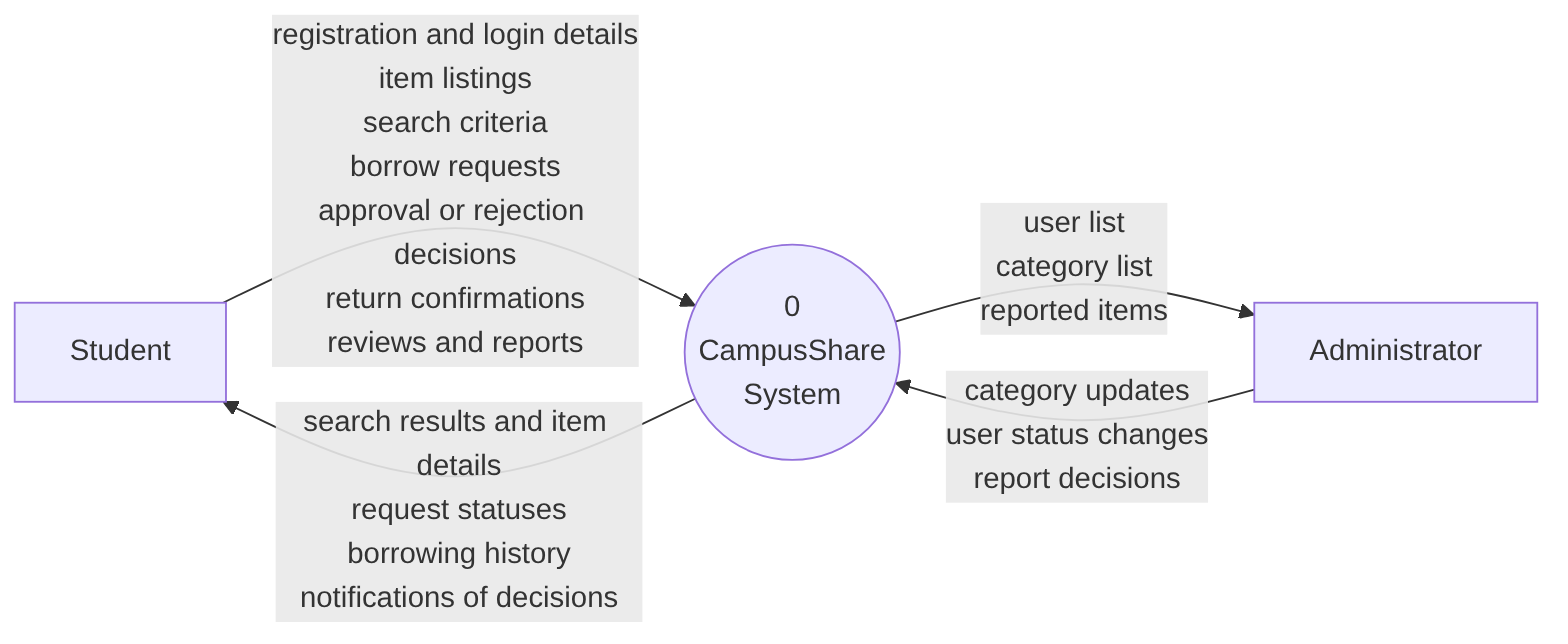
\includegraphics[width=0.95\textwidth]{dfd_context.png}
\caption{DFD context diagram (Level 0).}\label{fig:dfd0}
\end{figure}

\begin{figure}[H]
\centering
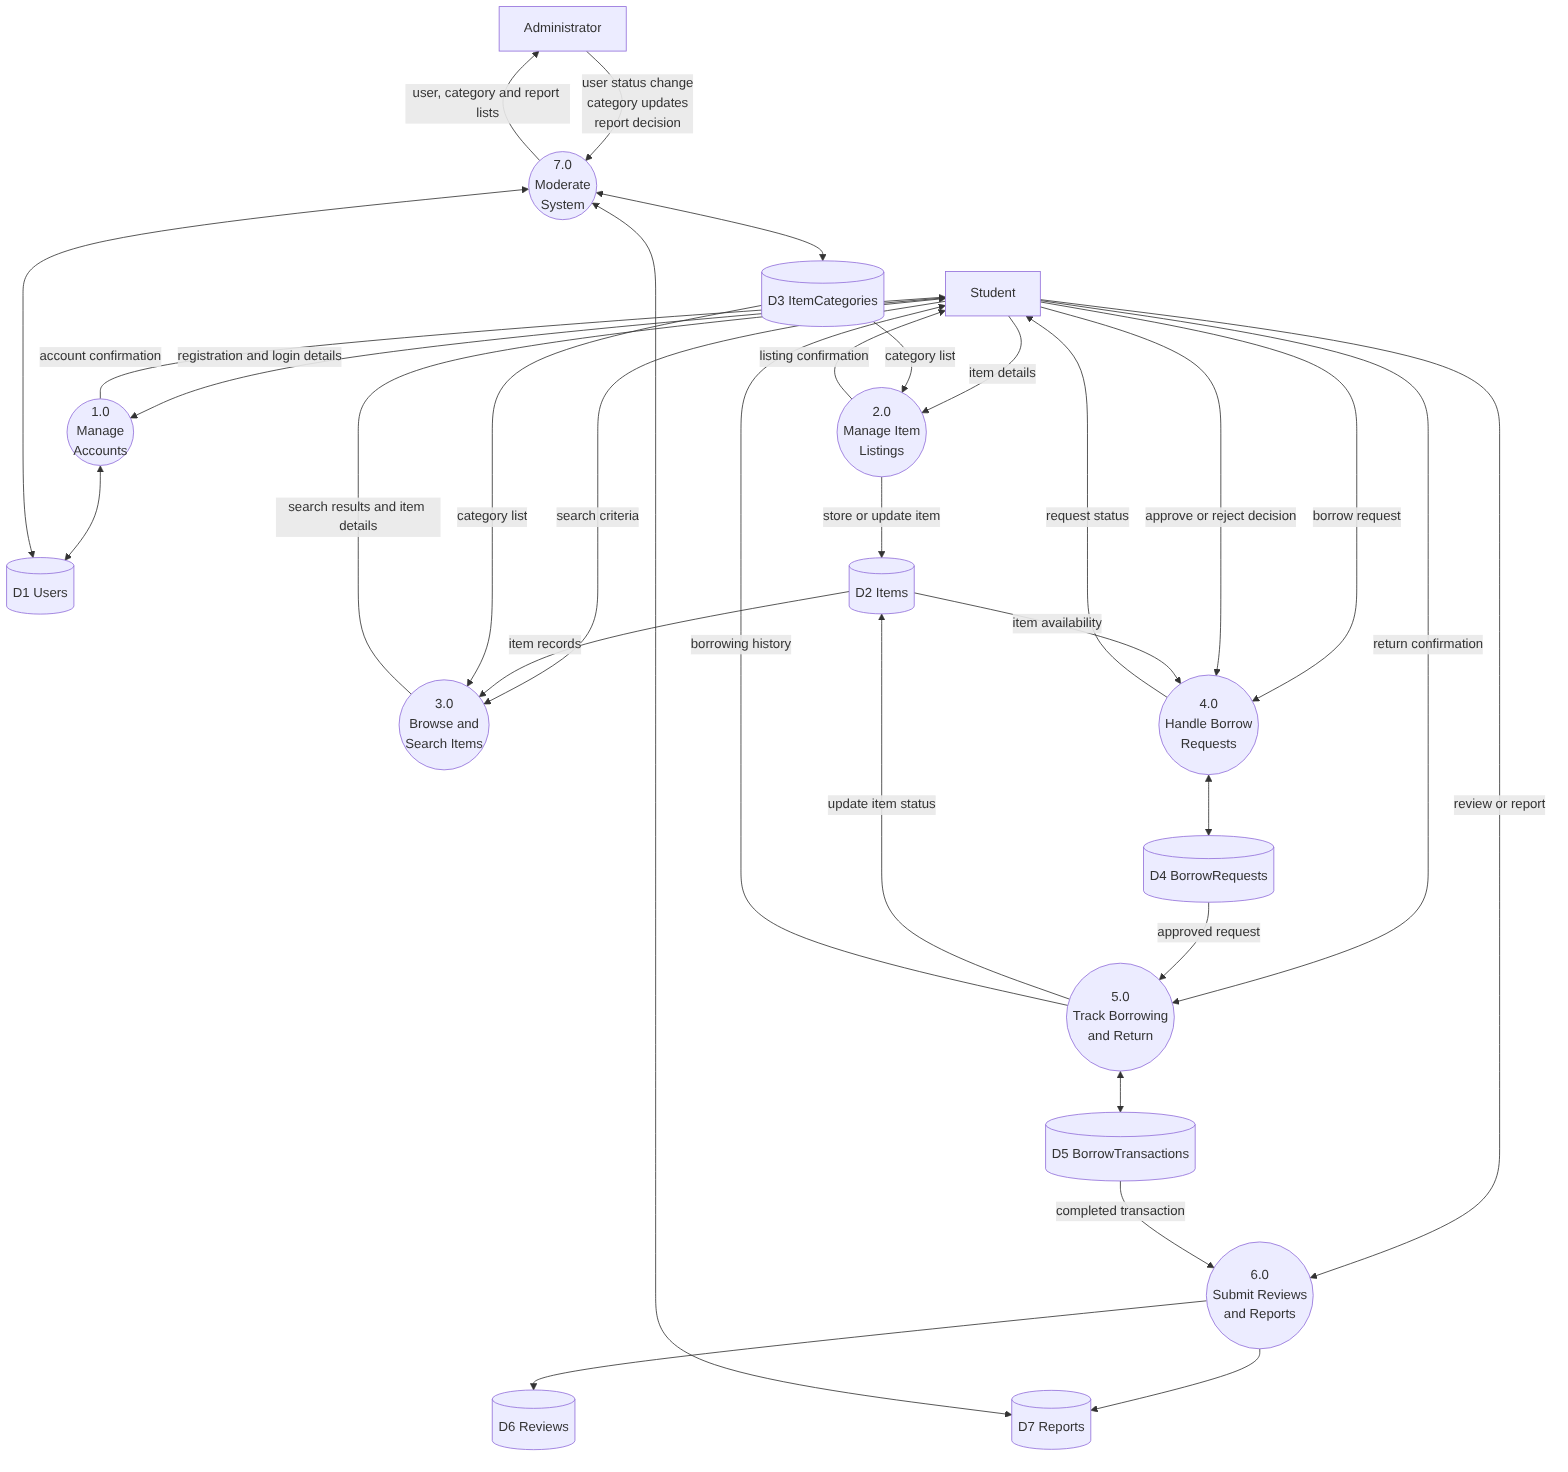
\includegraphics[width=\textwidth,height=0.82\textheight,keepaspectratio]{dfd_level1.png}
\caption{DFD Level 1: processes 1.0--7.0 and data stores D1--D7.}\label{fig:dfd1}
\end{figure}

\subsection{Use Case Diagram}
Figure~\ref{fig:usecase} shows the actions available to the Student and Administrator actors (source: \texttt{use\_case.puml}) \cite{fowler2003,omguml2017}.

\begin{figure}[H]
\centering
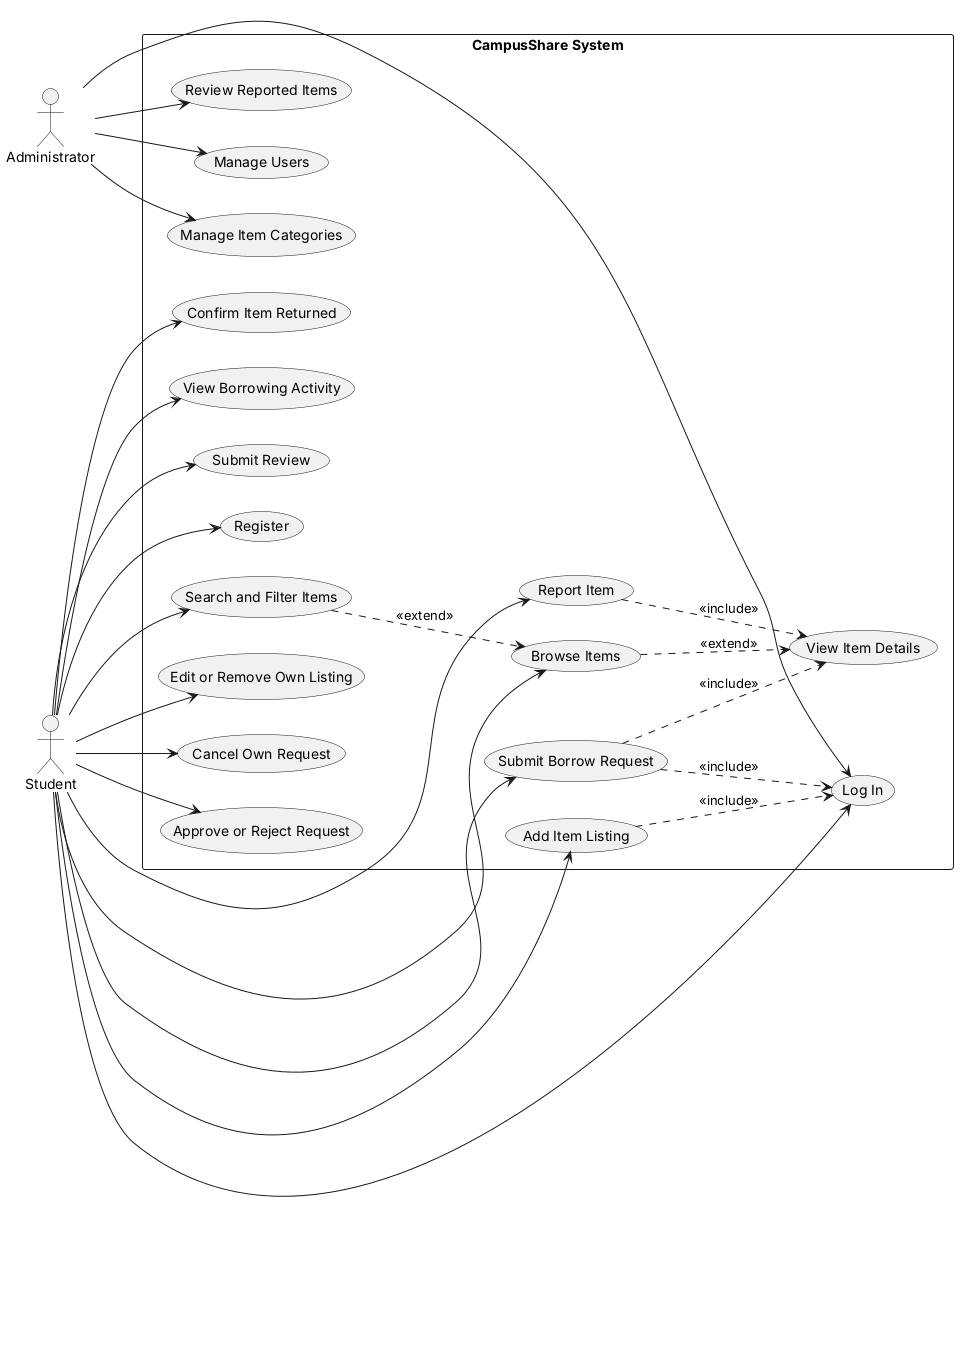
\includegraphics[width=\textwidth,height=0.7\textheight,keepaspectratio]{use_case.png}
\caption{UML use case diagram.}\label{fig:usecase}
\end{figure}

\subsection{Activity Diagram}
Figure~\ref{fig:activity} shows the borrowing process from browsing an item to return, including the approval or rejection decision (source: \texttt{activity.puml}).

\begin{figure}[H]
\centering
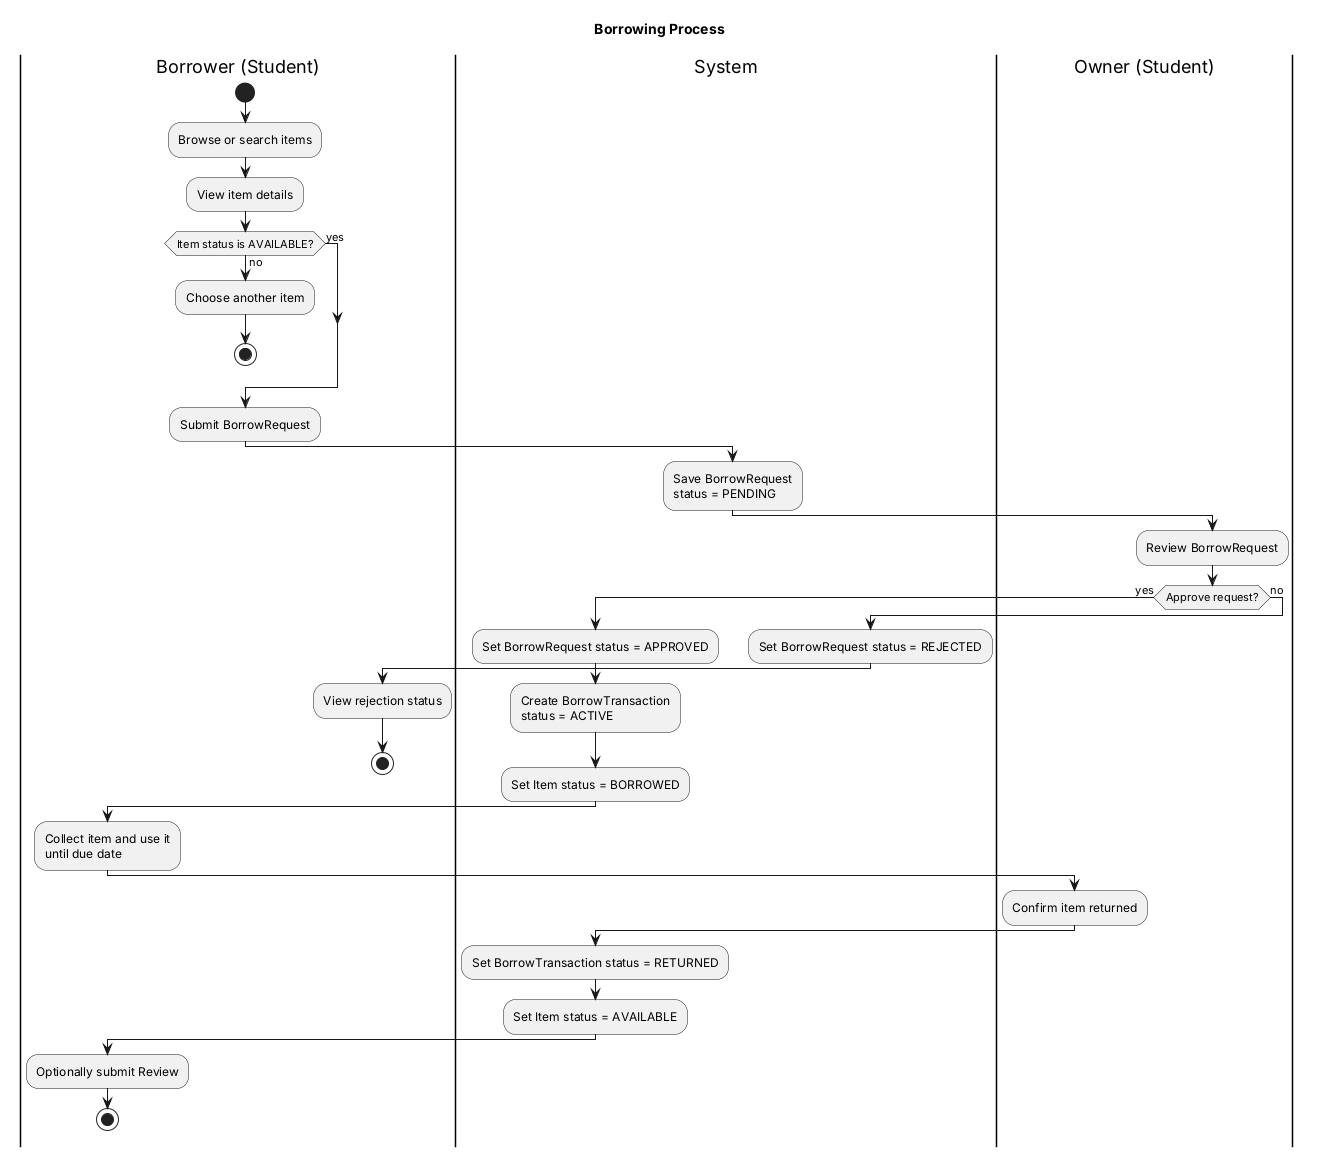
\includegraphics[width=\textwidth,height=0.8\textheight,keepaspectratio]{activity.png}
\caption{UML activity diagram of the borrowing process.}\label{fig:activity}
\end{figure}

\subsection{Entity Relationship Diagram (ERD)}
Figure~\ref{fig:erd} shows the database entities with primary keys (PK), foreign keys (FK), and relationships (source: \texttt{erd.mmd}).

\begin{figure}[H]
\centering
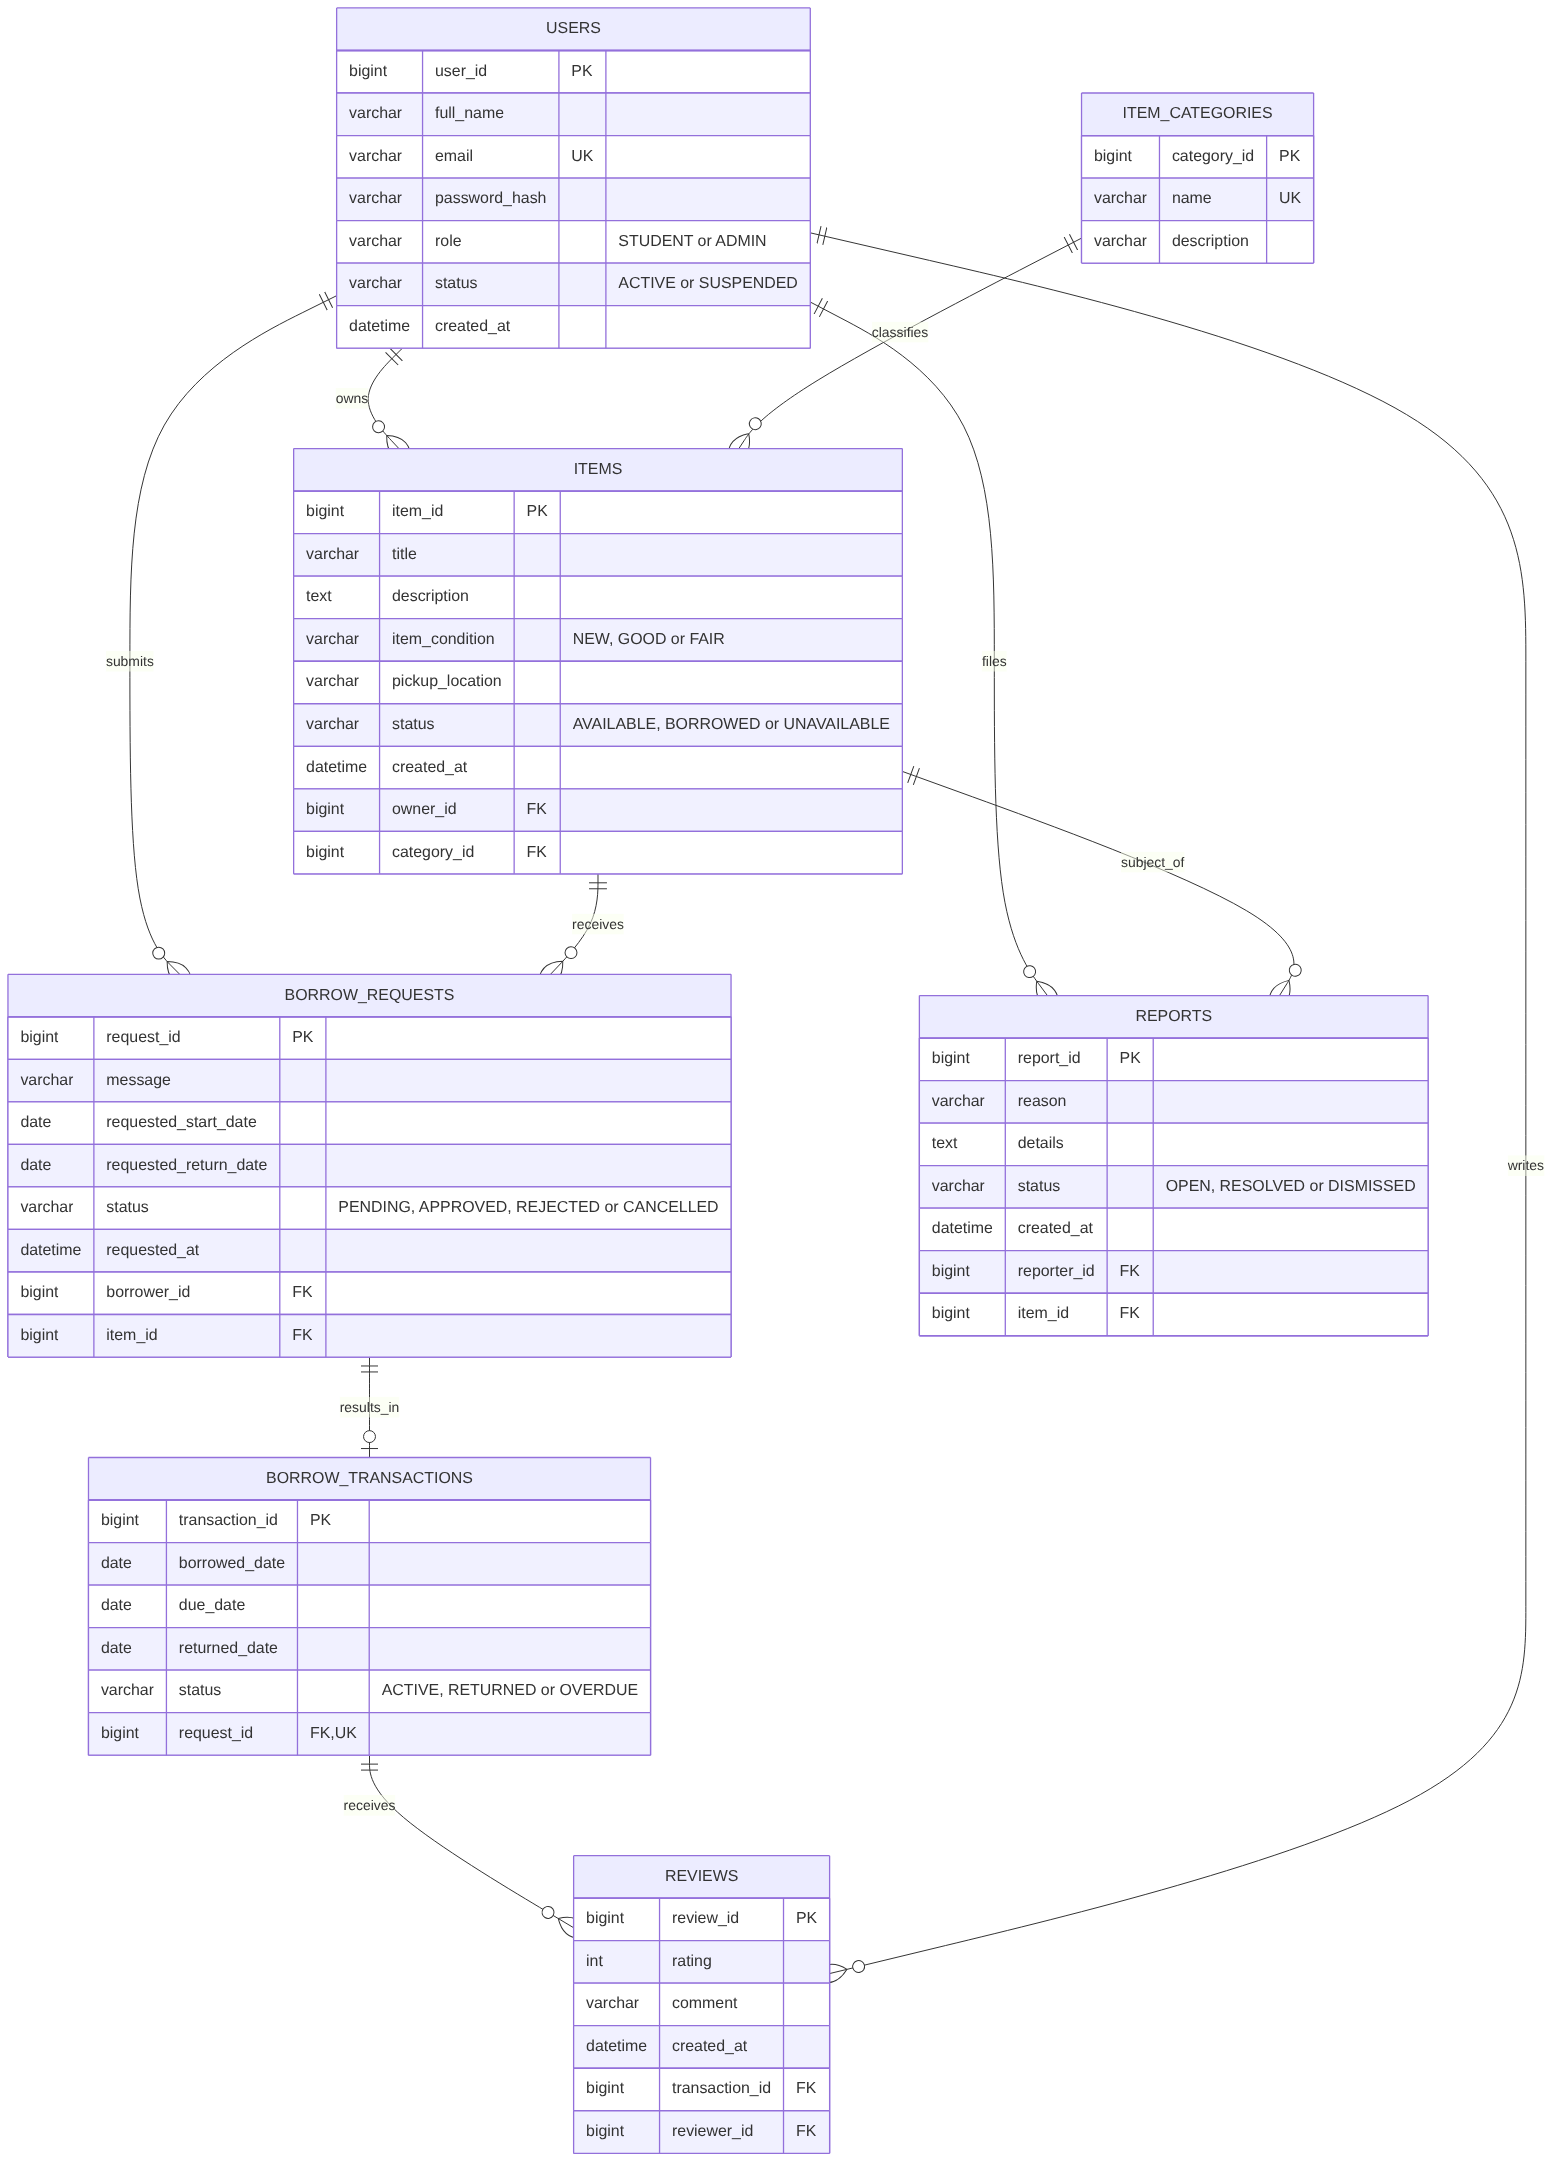
\includegraphics[width=\textwidth,height=0.82\textheight,keepaspectratio]{erd.png}
\caption{Entity relationship diagram.}\label{fig:erd}
\end{figure}

\subsection{Class Diagram}
Figure~\ref{fig:class} shows the seven domain classes (User, Item, ItemCategory, BorrowRequest, BorrowTransaction, Review, Report), their attributes, selected methods, multiplicities, and status enumerations (source: \texttt{class\_diagram.puml}).

\begin{figure}[H]
\centering
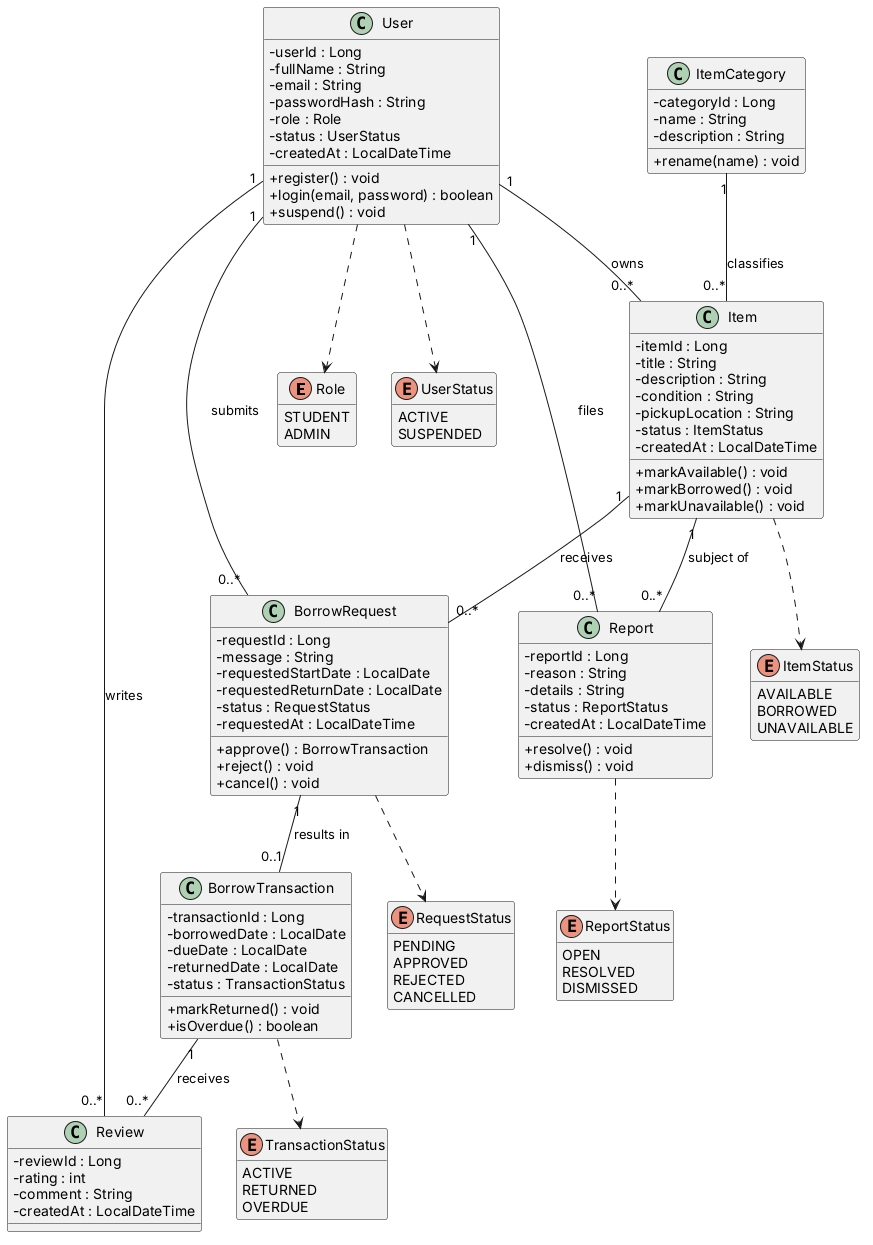
\includegraphics[width=\textwidth,height=0.82\textheight,keepaspectratio]{class_diagram.png}
\caption{UML class diagram of the domain model.}\label{fig:class}
\end{figure}

\subsection{Object Diagram}
Figure~\ref{fig:object} shows one example state of the system: Amina Rahman owns a calculator, Tanvir Hasan has an approved request for it, and an ACTIVE transaction exists (source: \texttt{object\_diagram.puml}). The values are sample data only.

\begin{figure}[H]
\centering
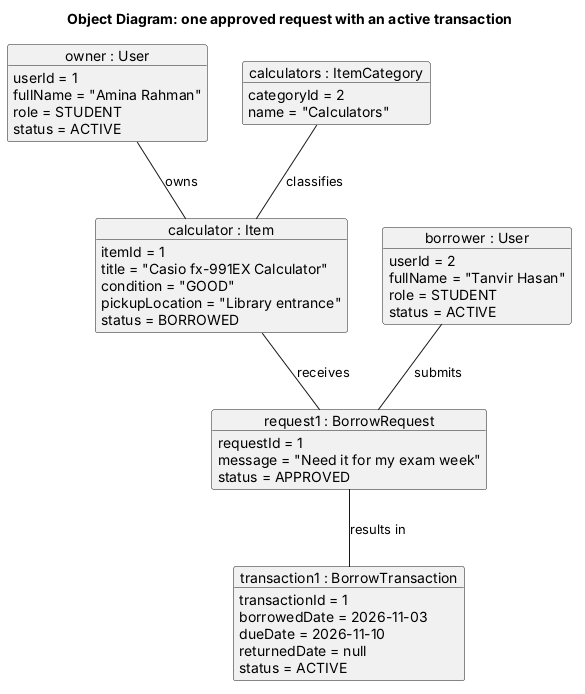
\includegraphics[width=\textwidth,height=0.6\textheight,keepaspectratio]{object_diagram.png}
\caption{UML object diagram (an instance snapshot, not a class model).}\label{fig:object}
\end{figure}

% ---------- 14 Database ----------
\section{Basic Database Design}
The MySQL database will contain seven tables that correspond to the domain classes. Table~\ref{tab:db} summarises them; the full structure is shown in the ERD.

\begin{table}[H]
\centering
\caption{Planned database tables.}\label{tab:db}
\begin{tabularx}{\textwidth}{@{}l l X@{}}
\toprule
\textbf{Table} & \textbf{Class} & \textbf{Key columns}\\
\midrule
users & User & user\_id (PK), full\_name, email (unique), password\_hash, role, status\\
item\_categories & ItemCategory & category\_id (PK), name (unique), description\\
items & Item & item\_id (PK), title, item\_condition, status, owner\_id (FK), category\_id (FK)\\
borrow\_requests & BorrowRequest & request\_id (PK), status, borrower\_id (FK), item\_id (FK)\\
borrow\_transactions & BorrowTransaction & transaction\_id (PK), due\_date, returned\_date, status, request\_id (FK, unique)\\
reviews & Review & review\_id (PK), rating, comment, transaction\_id (FK), reviewer\_id (FK)\\
reports & Report & report\_id (PK), reason, status, reporter\_id (FK), item\_id (FK)\\
\bottomrule
\end{tabularx}
\end{table}

% ---------- 15 UI prototype ----------
\section{UI Prototype Overview}
An initial prototype is provided in the \texttt{prototype/} folder, built with HTML, CSS, Bootstrap, and JavaScript. It uses fixed sample data held in the browser and \textbf{is not connected to a backend or database}. Login, saving, and borrowing actions are simulated for demonstration only.

\begin{table}[H]
\centering
\caption{Prototype screens and the domain classes they demonstrate.}
\begin{tabularx}{\textwidth}{@{}l X@{}}
\toprule
\textbf{Screen} & \textbf{Domain classes shown}\\
\midrule
Dashboard & User, Item, BorrowRequest, BorrowTransaction\\
Browse and search & Item, ItemCategory, User (owner)\\
Item details & Item, ItemCategory, User, Review, Report, BorrowRequest\\
Add or edit listing & Item, ItemCategory\\
Requests & BorrowRequest, Item, User, BorrowTransaction\\
My items and activity & Item, BorrowTransaction, BorrowRequest, Review\\
\bottomrule
\end{tabularx}
\end{table}

\subsection*{Implementation status}
\begin{tabularx}{\textwidth}{@{}l X l@{}}
\toprule
\textbf{Item} & \textbf{Description} & \textbf{Status}\\
\midrule
Proposal and design diagrams & This document and the diagram source files & Prepared\\
UI prototype & Static, simulated screens with sample data & Prepared\\
Spring Boot application & Controllers, services, repositories, entities & Planned\\
MySQL database & Schema and persistence & Planned\\
Real login and security & Authentication and role-based access & Planned\\
Testing & Test cases listed in this proposal & Planned\\
\bottomrule
\end{tabularx}

% ---------- 16 Schedule ----------
\section{Six-Week Development Schedule}
The schedule below is a \textbf{proposed plan for future work}. It does not mean that any of the listed development tasks, other than the proposal, diagrams, and prototype, have been completed. Relative weeks are used instead of calendar dates.

\begin{table}[H]
\centering
\caption{Task schedule.}
\small
\begin{tabularx}{\textwidth}{@{}l X c c c l@{}}
\toprule
\textbf{ID} & \textbf{Task} & \textbf{Start} & \textbf{End} & \textbf{Duration} & \textbf{Depends on}\\
\midrule
T1 & Requirements and proposal & W1 & W1 & 1 week & --\\
T2 & System design and UML diagrams & W1 & W2 & 1.5 weeks & T1\\
T3 & Database and project setup & W2 & W2 & 1 week & T2\\
T4 & Core item listing functionality & W3 & W3 & 1 week & T3\\
T5 & Borrowing request and approval workflow & W4 & W4 & 1 week & T4\\
T6 & UI integration & W4 & W5 & 1.5 weeks & T4, T5\\
T7 & Testing and debugging & W5 & W6 & 1.5 weeks & T5, T6\\
T8 & Documentation and final delivery & W6 & W6 & 1 week & T7\\
\bottomrule
\end{tabularx}
\end{table}

\begin{figure}[H]
\centering
\begin{ganttchart}[
  hgrid, vgrid,
  x unit=1.25cm, y unit chart=0.62cm, y unit title=0.6cm,
  title height=1, bar height=0.55,
  bar/.append style={fill=blue!55},
  milestone/.append style={fill=orange!85},
  bar label font=\footnotesize, milestone label font=\footnotesize,
  title label font=\footnotesize
]{1}{6}
\gantttitle{Week}{6}\\
\gantttitlelist{1,...,6}{1}\\
\ganttbar{T1 Requirements and proposal}{1}{1}\\
\ganttbar{T2 Design and UML diagrams}{1}{2}\\
\ganttbar{T3 Database and project setup}{2}{2}\\
\ganttbar{T4 Core item listing}{3}{3}\\
\ganttbar{T5 Request and approval workflow}{4}{4}\\
\ganttbar{T6 UI integration}{4}{5}\\
\ganttbar{T7 Testing and debugging}{5}{6}\\
\ganttbar{T8 Documentation and delivery}{6}{6}\\
\ganttmilestone{M1 Proposal ready}{1}\\
\ganttmilestone{M2 Design and DB ready}{2}\\
\ganttmilestone{M3 Increment 1 done}{3}\\
\ganttmilestone{M4 Increment 2 done}{4}\\
\ganttmilestone{M5 UI integrated}{5}\\
\ganttmilestone{M6 Final delivery}{6}
\end{ganttchart}
\caption{Proposed Gantt chart (relative weeks). Blue bars are tasks; orange diamonds are milestones.}
\end{figure}

% ---------- 17 Milestones ----------
\section{Milestones and Deliverables}
\begin{tabularx}{\textwidth}{@{}l c l X@{}}
\toprule
\textbf{ID} & \textbf{End of} & \textbf{Milestone} & \textbf{Deliverable}\\
\midrule
M1 & W1 & Proposal and requirements ready & Proposal document, requirements list\\
M2 & W2 & Design and database ready & Six diagrams, MySQL schema, Maven project skeleton\\
M3 & W3 & Increment 1 complete & Working item listing, browsing, and search\\
M4 & W4 & Increment 2 complete & Working request, approval, and return workflow\\
M5 & W5 & UI integrated & Thymeleaf pages for all main screens, reviews, reports, and admin pages\\
M6 & W6 & Final delivery & Tested application, final report, GitHub repository, README\\
\bottomrule
\end{tabularx}

% ---------- 18 Testing ----------
\section{Basic Testing Strategy}
Testing is planned for Weeks 5--6, with simple checks after each increment. The strategy includes:
\begin{itemize}
  \item \textbf{Unit tests} for service methods using JUnit (for example, approving a request);
  \item \textbf{Manual functional tests} of each workflow through the browser;
  \item \textbf{Basic validation tests} for forms and role-based access.
\end{itemize}
Table~\ref{tab:tests} lists example test cases. They are planned and have not yet been run.

\begin{table}[H]
\centering
\caption{Example planned test cases.}\label{tab:tests}
\small
\begin{tabularx}{\textwidth}{@{}l X X@{}}
\toprule
\textbf{ID} & \textbf{Test} & \textbf{Expected result}\\
\midrule
TC-01 & Register with an already used email & Registration is rejected with a message\\
TC-02 & Add a listing with an empty title & Form shows a validation error\\
TC-03 & Search items by keyword ``calculator'' & Only matching items are listed\\
TC-04 & Request an item with status BORROWED & Request is not allowed\\
TC-05 & Owner approves a PENDING request & Request becomes APPROVED, an ACTIVE BorrowTransaction is created, and the item becomes BORROWED\\
TC-06 & Owner confirms return & Transaction becomes RETURNED and the item becomes AVAILABLE\\
TC-07 & Student opens an admin page & Access is denied\\
\bottomrule
\end{tabularx}
\end{table}

% ---------- 19 Risks ----------
\section{Risk Analysis and Mitigation}
\begin{tabularx}{\textwidth}{@{}l X c X@{}}
\toprule
\textbf{ID} & \textbf{Risk} & \textbf{Level} & \textbf{Mitigation}\\
\midrule
R1 & Limited time for one developer & High & Keep scope small; build the core workflow first; cut optional features if needed.\\
R2 & Difficulty with Spring Boot or JPA & Medium & Follow official documentation; build small examples early in Week 2.\\
R3 & Workflow errors in request statuses & Medium & Define status rules in the diagrams; write unit tests for the service layer.\\
R4 & Data loss or code loss & Medium & Commit to GitHub regularly; keep a database script.\\
R5 & Security mistakes in login or access & Medium & Hash passwords; use role checks; validate inputs.\\
R6 & Last-week delays & Medium & Reserve Week 6 for testing and documentation only.\\
\bottomrule
\end{tabularx}

% ---------- 20 Expected outcomes ----------
\section{Expected Outcomes}
At the end of the planned development, the project is expected to deliver:
\begin{itemize}
  \item a working web application for listing, browsing, requesting, and returning campus items;
  \item an administrator interface for users, categories, and reports;
  \item a MySQL database design consistent with the ERD and class diagram;
  \item a tested core workflow and a documented GitHub repository;
  \item a final report describing the design, implementation, and testing.
\end{itemize}
These outcomes are targets of the plan and depend on completing the proposed schedule.

% ---------- 21 Conclusion ----------
\section{Conclusion}
CampusShare addresses a small but practical problem: organising item sharing among students. The project is limited in scope, uses well-documented technologies, and is divided into increments suitable for one student over six weeks. This proposal provides the requirements, six design diagrams, database design, schedule, and an initial prototype as a base for the implementation phase.

% ---------- 22 References ----------
\bibliographystyle{plain}
\bibliography{references}
\addcontentsline{toc}{section}{References}

\end{document}
